\newpage
\section{Określenie wymagań szczegółowych}		%2


Nasza aplikacja motywacyjna to nowoczesne narzędzie, zaprojektowane z myślą o wspieraniu użytkowników w codziennym dążeniu do realizacji ich celów. Wykorzystując najnowsze technologie, takie jak .NET MAUI do budowy interfejsu użytkownika, Firebase do zarządzania danymi oraz dodatkowe funkcje, takie jak aparat, GPS i biometria, aplikacja zapewnia stabilność, bezpieczeństwo.


\textbf{\large{Technologie:} } .NET MAUI i XML – Używamy MAUI do tworzenia aplikacji na różne platformy (iOS, Android, Windows, macOS), co zapewnia spójny wygląd i funkcjonalność. Interfejs zaprojektowany w XML jest przejrzysty i dostosowany do intuicyjnego użytkowania.

    \textbf{Firebase}– Wspomaga synchronizację danych użytkownika, zarządzanie powiadomieniami oraz autoryzację. Dane przechowywane w chmurze są dostępne z każdego urządzenia.

 

    \\
      \textbf{\large{ Czujniki i urządzenia:} } Aparat – Aplikacja pozwala na wykorzystanie aparatu do dokumentowania postępów, np. w zakresie poprawy kondycji fizycznej. Użytkownicy mogą robić zdjęcia „przed” i „po” w trakcie swoich wyzwań, co dodatkowo motywuje do dalszych działań.
       \GPS– W przypadku wysyłania spersonalizowanych powiadomień, na przykład w czasie gdy pogoda nie dopisuje.
        Biometria– Aby zwiększyć bezpieczeństwo, aplikacja wspiera logowanie przy użyciu biometrii, takiej jak odcisk palca czy rozpoznawanie twarzy. Pozwala to na szybki i bezpieczny dostęp do danych użytkownika, bez konieczności pamiętania haseł.

\textbf{{\large Funkcje aplikacji:}}

    Cele i zadania – Użytkownicy mogą ustalać cele i dzielić je na mniejsze kroki. Aplikacja przypomni o kolejnych zadaniach, a postępy są bezpiecznie przechowywane i synchronizowane z Firebase.

    Powiadomienia motywacyjne – Aplikacja wysyła inspirujące wiadomości dostosowane do harmonogramu użytkownika i jego postępów. Wykorzystuje Firebase do przechowywania bazy cytatów.

    Śledzenie postępów z wykorzystaniem  aparatu – Dla celów związanych z poprawą stanu swojej sylwetki użytkownicy mogą tworzyć dokumentacji wizualnej postępów, np. zdjęć „przed” i „po”. Wszystkie dane są przechowywane i synchronizowane w Firebase, co umożliwia dostęp do nich z każdego urządzenia.

    Logowanie biometryczne – W trosce o bezpieczeństwo użytkowników, aplikacja wspiera logowanie biometryczne (odcisk palca), które pozwala na szybki i bezpieczny dostęp do danych osobistych.

    Synchronizacja i bezpieczeństwo danych – Firebase zapewnia bezpieczne przechowywanie danych, które są synchronizowane na wszystkich urządzeniach użytkownika. Dzięki biometrii dostęp do aplikacji jest chroniony, a logowanie jest proste i szybkie.





%rysunek 1
	\begin{figure}[!htb]
	\begin{center}
		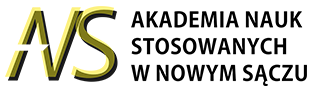
\includegraphics[width=8cm]{rys/ans.png}
		\caption{Szkic interfejsu graficznego}
		\label{rys:rysunek001}
	\end{center}
\end{figure}





%Dokładne określenie wymagań aplikacji (cel, zakres, dane wejściowe) – np. opisać przyciski, czujniki, wygląd layautu, wyświetlenie okienek. Opisać zachowanie aplikacji – co po kliknięciu, zdarzenia automatyczne. Opisać możliwość dalszego rozwoju oprogramowania. Opisać zachowania aplikacji w niepożądanych sytuacjach.



